\section{Application and Comparison}
This chapter covers the application of random forest regression and the evaluation of its performance.

In \autoref{sec:simulation}, we apply the random forest on simulated data, 
and show how its performance develops over increasing sample sizes.

Then in \autoref{sec:real_data}, we apply the random forest on the real Titanic data set \cite{titanicData}
and evaluate its performance.

In \ref{sec:adaboost} and \ref{sec:gradient_boosting}, we apply AdaBoost and Gradient
Boosting respectively on the Titanic data set and  compare their performance with that of the random forest.

\subsection{Application of Random Forest on simulated data}
\label{sec:simulation}

In the simulation, we use a linear and a non-linear data generating process (DGP) for random forest regression.
The linear DGP generates the data tuples \( (y, x_{1}, x_{2}, x_{3}) \) as follows:

\begin{equation}\label{eq:linear_dgp}
    y = \beta_{0} + \beta_{1} x_{1} + \beta_{2} x_{2} + \beta_{3} x_{3} + \epsilon,
\end{equation}

whereas \( (\beta_{0}, \beta_{1}, \beta_{2}, \beta_{3}) = (0.3, 5, 10, 15) \),
\( x_{1}, x_{2}, x_{3} \sim \mathcal{N}(0,\,3) \), and \( \epsilon \sim \mathcal{N}(0,\,1) \).

The performance of the Random Forest over an increasing sample is illustrated
below in \autoref{fig:forest_vs_ols_linearDGP} and \autoref{fig:forest_vs_ols_nonLinearDGP}.
For each sample drawn from the linear DGP, a set of parameters
were optimized via cross validation. Then, the residual sum of squares (RSS) gets calculated
based on the holdout set of 100 instances.

\begin{figure}
    \captionsetup{format=plain}
    \makebox[\textwidth]{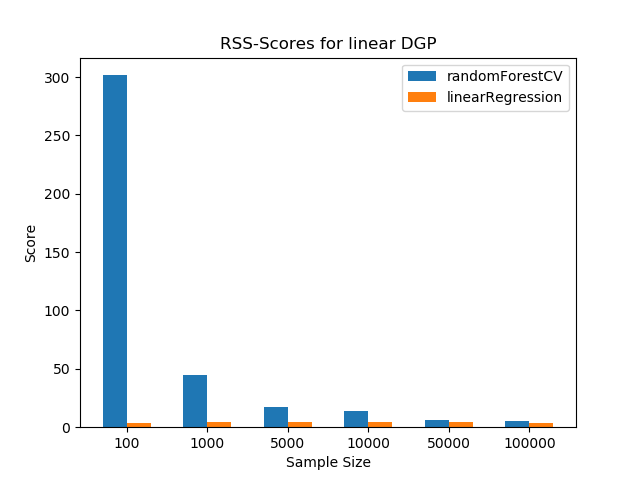
\includegraphics[width=120mm]{forest_vs_ols_linearDGP.png}}
    \caption
        {This plot illustrates the RSS for different training sample sizes for Random Forest and OLS.
        These samples where drawn from a linear DGP in accordance to \autoref{eq:linear_dgp}.
        The holdout set for calculating the RSS were drawn again for each training sample from the same DGP.
        It always contained 100 observations. In case of the Random Forest, for each sample the parameters
        got optimized again via cross validation.
        }
    \label{fig:forest_vs_ols_linearDGP}
\end{figure}

As one can see in \autoref{fig:forest_vs_ols_linearDGP}, the RSS of the Random Forest converges for the linear DGP
to that of the OLS for increasing sample sizes. 

The non-linear DGP generates the data tuples \( (y, x_{1}, x_{2}) \) as follows:

\begin{equation}\label{eq:non_linear_dgp}
    y = \beta_{0} + \beta_{1} I(x_{1} >= 0, x_{2} >= 0) + \beta_{2} I(x_{1} >= 0, x_{2} < 0) + \beta_{3} I(x_{1} < 0) + \epsilon,
\end{equation}

whereas \( (\beta_{0}, \beta_{1}, \beta_{2}, \beta_{3}) \), \( x_{1}, x_{2} \) and \(  \epsilon \)
are the same in the previous DGP.

\begin{figure}[H]
    \captionsetup{format=plain}
    \makebox[\textwidth]{\includegraphics[width=120mm]{forest_vs_ols_nonLinearDGP.png}}
    \caption
        {This plot illustrates the RSS for different training sample sizes for Random Forest and OLS.
        These samples where drawn from a non-linear DGP in accordance to \autoref{eq:non_linear_dgp}.
        The holdout set for calculating the RSS were drawn again for each training sample from the same DGP.
        It always contained 100 observations. In case of the Random Forest, for each sample the parameters
        got optimized again via cross validation.
        }
    \label{fig:forest_vs_ols_nonLinearDGP}
\end{figure}

As one can see above in \autoref{fig:forest_vs_ols_nonLinearDGP}, the Random Forest performs strictly better
than the OLS for any sample size. Due to this DGP resembling a stratification similar to
that of a Descision Tree, the RSS of the Random Forest converges relatively quickly while that of the OLS
remains unstable and high. 


\subsection{Application of Random Forest on real data}
\label{sec:real_data}
As previously mentioned, we applied the Random Forest on the Titanic data set \cite{titanicData} in order
to determine the survival of the passengers based on reported attributes like name title or booked cabin.
A major reason for choosing this data set was due to the fact that it consists of many categorical features.
In order to use the data to its fullest extent, we conducted additional feature engineering. 
Without that, many features remain unusable for our methods, 
because they contain missing values or values that are formatted as text.
For the implementation of the feature engineering and the classification,
one can consult our code repository \cite{githubApplication}.
The Random Forest managed to achieve a total classification accuracy of 84,32\% on the holdout set,
which consists out of 15\% of the total data.
According to the confusion matrix in \autoref{fig:confusion_matrix}, for passengers that died, 
the accuracy was slightly higher compared to those that survived. This is to be expected,
since deaths outnumber survivals considerably.

\begin{figure}[H]
    \captionsetup{format=plain}
    \makebox[\textwidth]{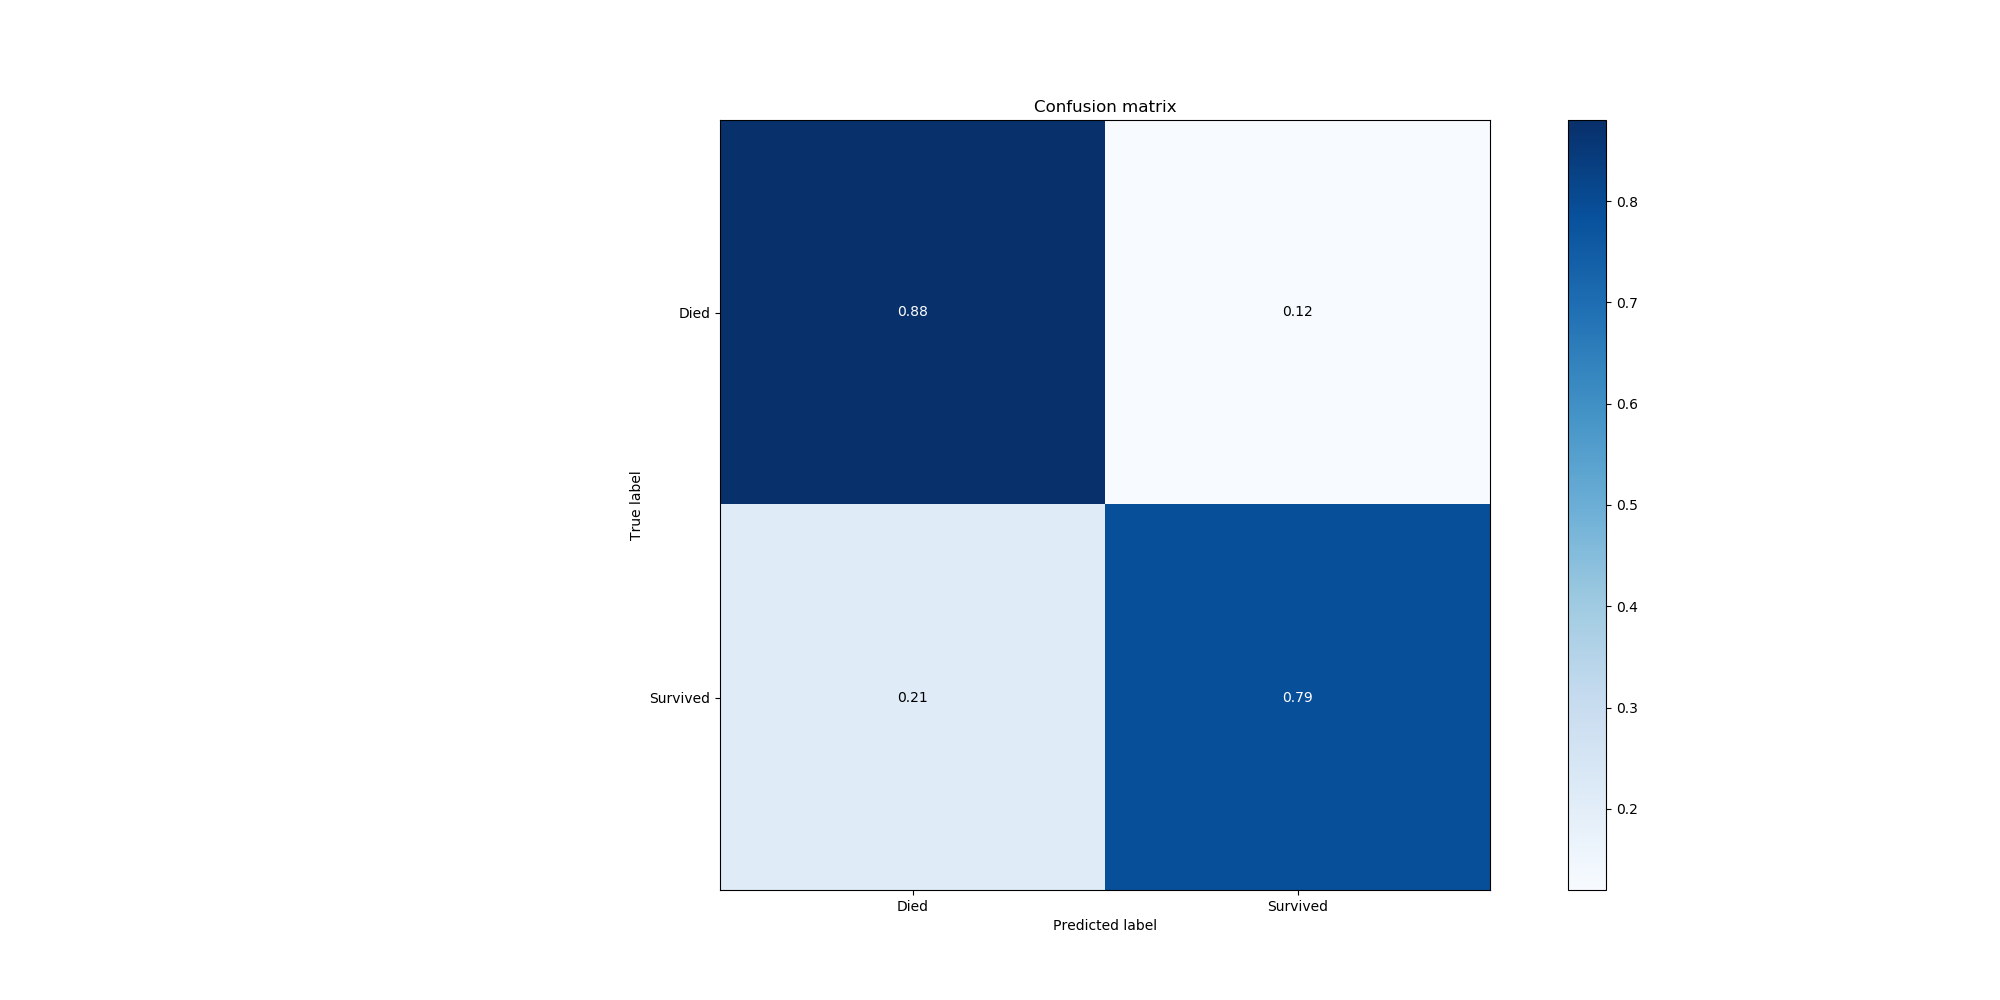
\includegraphics[width=200mm]{confusion_matrix.png}}
    \caption
        {This plot illustrates the accuracy of the Random Forest's prediction on the Titanic data set.
        }
    \label{fig:confusion_matrix}
\end{figure}


\section{Comparison to two boosting methods}
Before introducing AdaBoost and Gradient Boosting methods firstly, it is essential to understand what boosting is. Like bagging, boosting is an approach which can be applied to many machine learning methods for classification or regression. Bagging uses bootstrap to create multiple datasets for training the method. As a next stage bagging fits a separate decision tree to each training dataset, and then it combines all decision trees in order to create a single predictive model. Every decision tree is independent to others thanks to using bootstrap to create different training datasets. Boosting method works similarly, but in our case decision trees are grown sequentially. It means that each tree is built using information from previously built trees. Boosting method does not involve bootstrap sampling. In this method instead of bootstrap each decision tree is fit on a modified version of the original dataset \cite{James2013}.

\subsection{AdaBoost Classifier}
\label{sec:adaboost}

\subsubsection{An introduction to the AdaBoost method}
Adaptive Boosting (Adaboost) was introduced by \cite{freund1997boosting} and we employ Adaboost as a comparison 
technique against Random Forest. In the Adaboost algorithm, instead of fully-grown trees as in Random Forest, 
we use trees with only one internal node and two leaves also called stumps. We consider those as weak-learners 
compared to trees since its depth and power is limited. Before generating stumps, 
we assign weights to observations in the sample, normally the weight of each observation takes the value 
of $1/N$ as $N$ is the sample size. We generate a stump for each classifier in the data and compare them regarding 
their misclassification rate. After selecting the best classifier, with using its stump's misclassification rate 
we compute its stump's significance. With that significance, we compute new weights for the sample. 
We repeat the algorithm sequentially for the sample with new weights until a stopping criterion is achieved. 
Generally, using the number of classifiers as the number of iteration is a common practice (Elements of statistical learning). 
After generating multiple stumps, we can predict an observation's class. 
We get the decision of every stump and form groups accordingly. 
Every outcome class has a group of stumps which predict that class and every stump has its significance. 
After summing significance values of stumps in each group, the prediction is the class with the total highest significance. 
Although stumps are weak-learners, we exploit the error of a weak-learner to generate another weak-learner 
and iterating multiple times provides us with a powerful algorithm.

\subsubsection{Real Data Application of Adaboost}
When we employ Adaboost to predict the survival outcome of the passenger on Titanic, we achieve approximately a rate of 82\% accuracy. With utilizing the confusion matrix of Adaboost and compare it with Random Forest's, we can see that for the non-survivals the result is almost the same but Random Forest is better when it comes to identify survivors.

\begin{figure}[H]
    \captionsetup{format=plain}
    \makebox[\textwidth]{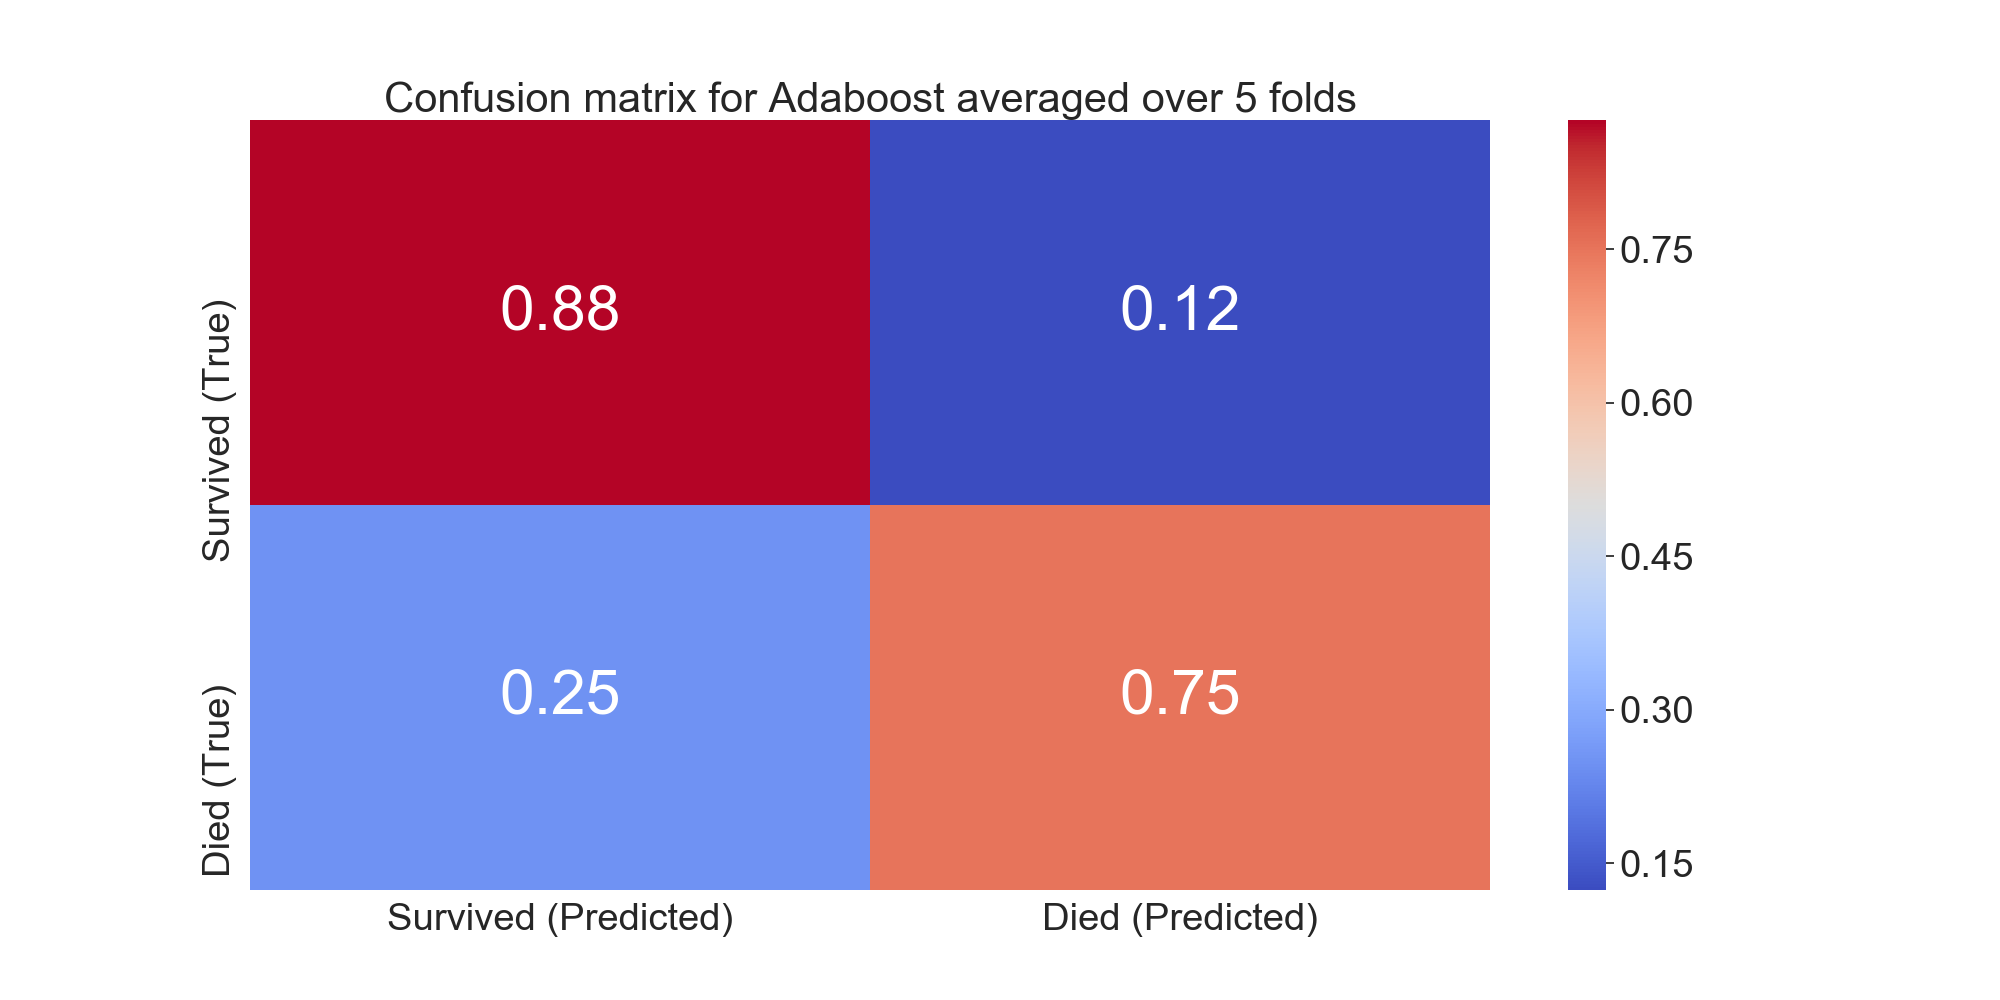
\includegraphics[width=200mm]{confusion_matrix_adaboost.png}}
    \caption
        {This plot illustrates the accuracy of the Adaboost's prediction on the Titanic data set.
        }
    \label{fig:confusion_matrix_adaboost}
\end{figure}


\subsection{Gradient Boosting Classifier}
\label{sec:gradient_boosting}

\subsubsection{An introduction to the Gradient Boosting method}
In Gradient Boosting the idea is to take weak learning algorithm or hypothesis and make some corrections that will improve the power of this algorithm/hypothesis. In hypothesis boosting, we check every observation on which statistical learning method was trained on, then you leave the observations which were correctly classified. Then method creates new weak learner and test it only on the observations that were poorly classified. Next, the examples that were correctly classified are kept.
The idea described above was used in the AdaBoost algorithm. In this algorithm, many weak learners are created by many decision trees that only have a single split. Created instances in the training dataset are weighted in the way that larger weights are assigned to instances which were difficult to classify. To the most difficult training instances weaker learners are added sequentially.
Gradient boosting classifiers are the Adaptive Boosting method, but it is combined with weighted minimization. After weighted minimization, all classifiers and weighted inputs are again calculated. The aim of gradient boosting classifiers is to minimize the loss and it operates in the similar way, as gradient descent in a neural network.
\subsubsection{Real data example}

After a simple and short introduction it is time to apply Gradient Boosting Classifier on the Titanic data set. As in every application in the paper,
after conducting feature engineering, we try to determine the survival of the passengers using available explanatory variables. 
Gradient Boosting Classifier if it comes to a total classification accuracy is slightly worse than the Random Forest method. In this case achieved accuracy is equal
approximately 82,84\%. 
As for the Random Forest, the confusion matrix in Figure 6
shows higher accuracy for passengers that died than passengers who survived and it is respectively 85\% and 80\%.


\begin{figure}[H]
    \captionsetup{format=plain}
    \makebox[\textwidth]{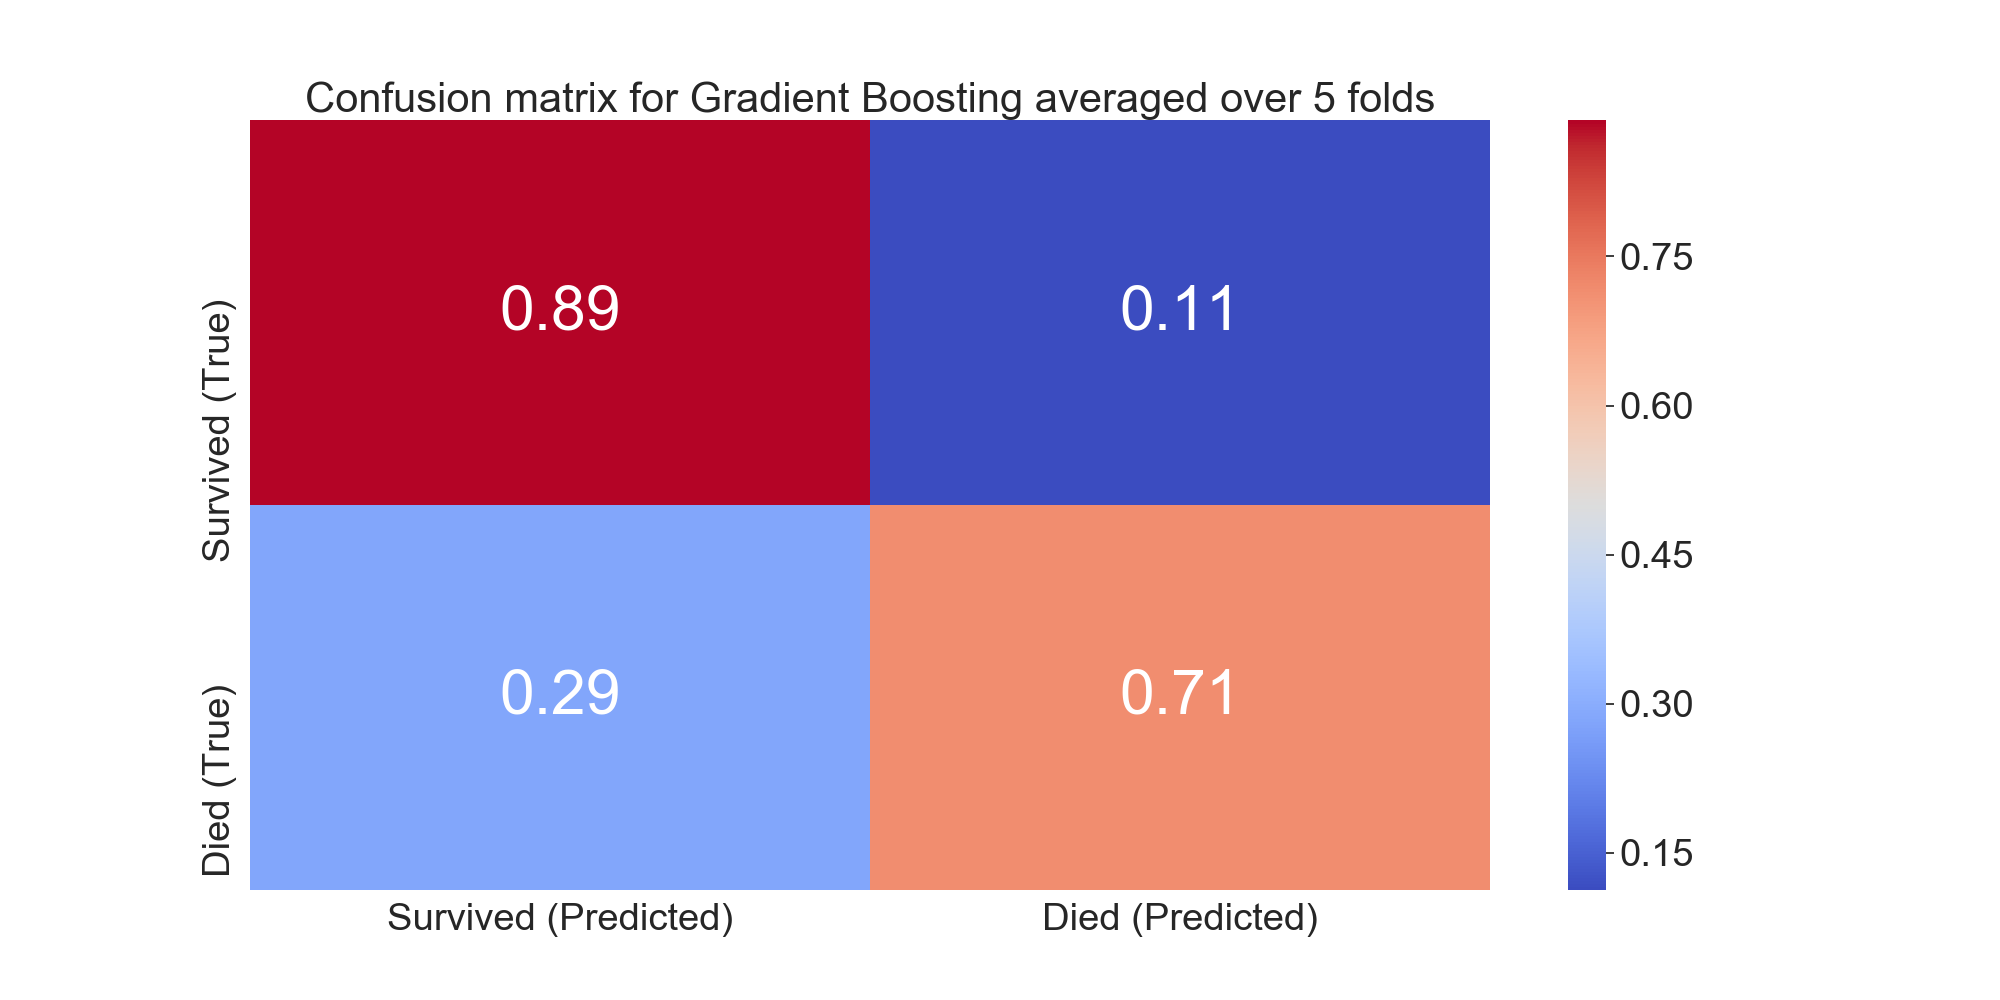
\includegraphics[width=200mm]{confusion_matrix_gradient_boosting.png}}
    \caption{This plot illustrates the accuracy of the Gradient Boosting Classifier's prediction on
             the Titanic data set.}
    \label{fig:confusion_matrix_gradient_boosting}
\end{figure}

